\chapter{Introduction}\label{ch:intr}
The phenomena of heavy-tailedness is widely observed in many
disciplines of science, for example, phase transition of matter and
black body radiation as studied in physics, neuronal avalanches in
biology, claim sizes of insurance mathematics and stock returns in
finance. The last application is indeed the focus of this thesis. To
discuss the phenomena in precise terms, we introduce the concept of
regular variation.

\section{Regular Variation}
The concept of regular variation is defined by the following scaling
property: if a function $f$ on $(0, \infty)$ satisfies
\[
\lim_{x \to \infty} {f(c x) \over f(x)} = c^\alpha
\quad
\forall c > 0
\]
then we say $f$ is regularly varying with index $\alpha$.
$f$ can be written in the form $f(x) = {L(x) \over x^\alpha}$, where
$L(x)$ is a slowly varying function, i.e.
$\lim_{x \to \infty} {L(c x) \over L(x)} = 1$, $\forall c > 0$.
We call a random variable $X$ regularly varying with index
$\alpha \geq 0$ if it satisfies the tail balance condition
\[
\P(X > x) \sim p_+ {L(x) \over x^\alpha},\quad
\P(X < -x) \sim p_- {L(x) \over x^\alpha}, \quad
\text{for some } p_+, p_- > 0,\; p_+ + p_- = 1
\]

% Distribution functions, say $F(\cdot)$, whose survival function
% $\bar F(x) = 1 - F(x)$ satisfies the above scaling property, are
% observed in a variety of phenomena, 
When expanded to multiple dimensions, the scaling property of regular
variation is better described in terms of vague convergence to a
spectral measure $\mu_\alpha$: if a random vector $V$ satisfies
\[
{
  \P(V/|V| \in \cdot, |V| > c x)
  \over
  \P(|V| > x)
}
\overset{v}{\to} c^{-\alpha} \mu_\alpha(\cdot)
\quad
x \to \infty, \forall c > 0,
\]
then we say $V$ is regularly varying with index $\alpha$. Here
$\mu_\alpha$ is a probability measure on the unit sphere
\cite{buraczewski:damek:mikosch:2016}. Clearly, if $V$
is regularly varying with index $\alpha$, then each component
and each linear combination of its components are regularly
varying with the same index $\alpha$. This follows from Feller
\cite{feller}, p. 278. Cf. also Jessen and Mikosch
\cite{JessenMikosch2006}, lemma 3.1, and Embrechts et. al.
\cite{embrechts:klueppelberg:mikosch:1997}, lemma 1.3.1.

Clearly, estimating the tail index $\alpha$ of a sequence
$X_1, X_2, \dots$ of regularly varying variables is particularly
important for understanding the behaviour of a heavy-tailed series. A
standard method proposed for this purpose is due to Hill
\cite{hill1975simple}:
\begin{equation}
  \label{eq:fhhty}
  \hat \alpha_H = \left[
    {1 \over k} \sum_{i=1}^k \log \left(
      X_{(i)} \over X_{(k+1)}
    \right)
  \right]^{-1}
\end{equation}
where $X_1, X_2, \dots, X_n$ is a sample whose tail index is the
subject of estimation, and $X_{(i)}$ is the $i$-th upper order
statistic of the sample. Several authors have contributed to showing
the weak consistency and asymptotic normality of the estimator
$\hat \alpha_H$, under the assumptions $k \to \infty, k/n \to 0$
as $n \to \infty$.

%% Mason \cite{mason:1982} first proved that the estimator
%% was consistent when $X_1, X_2, \dots$ were iid; later Rootz\'en,
%% Leadbetter and de Haan \cite{rootzen:leadbetter:dehaan1992} and Hsing
%% \cite{hsing:1991} proved its consistency when $X_1, X_2, \dots$ were
%% weakly dependent; and Resnick and St{\u a}ric{\u a}
%% \cite{resnick:starica:1995, resnick:starica:1997} proved its
%% consistency when $X_t$ was a linear process.

Figure \ref{fig:thjyuj} shows the Hill estimates of the tail indices
of daily stock return series from 3 sectors of the
{\em Standard \& Poor 500} index \footnote{An American stock index
  comprising 500 or so companies.}. The 2.5\% and 97.5\% quantiles of
the asymptotic normal distribution of the estimates are also
given. One can see the confidence bands are fairly large compared with
the estimated values. This certainly raises the question of how
similar they really are and if/how their variations can be explained by
economical arguments. We explore this topic in chapter
\ref{ch:TailParameters}.

\begin{figure}[htb!]
  \begin{minipage}{1.0\linewidth}
    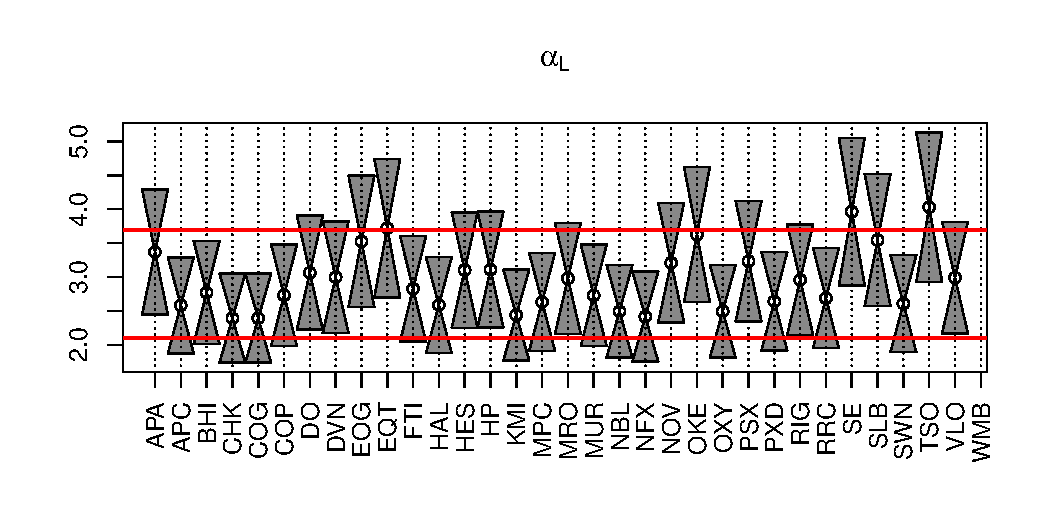
\includegraphics[width=\textwidth, trim={0, 0.8cm, 0, 2cm}, clip]
    {Energy_lower.pdf}
  \end{minipage}
  \begin{minipage}{1.0\linewidth}
    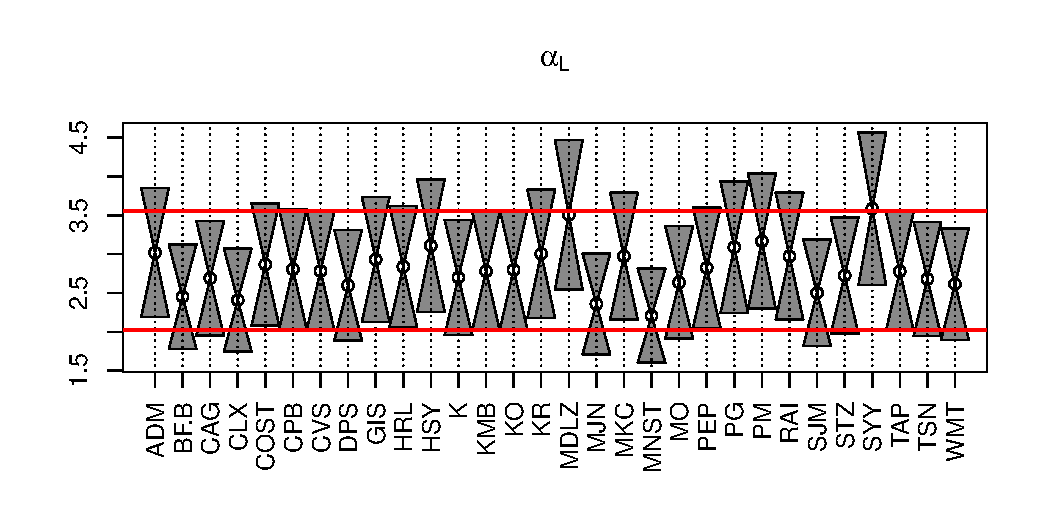
\includegraphics[width=\textwidth, trim={0, 0.8cm, 0, 2cm}, clip]
    {Consumer_Staples_lower.pdf}
  \end{minipage}
  \begin{minipage}{1.0\linewidth}
    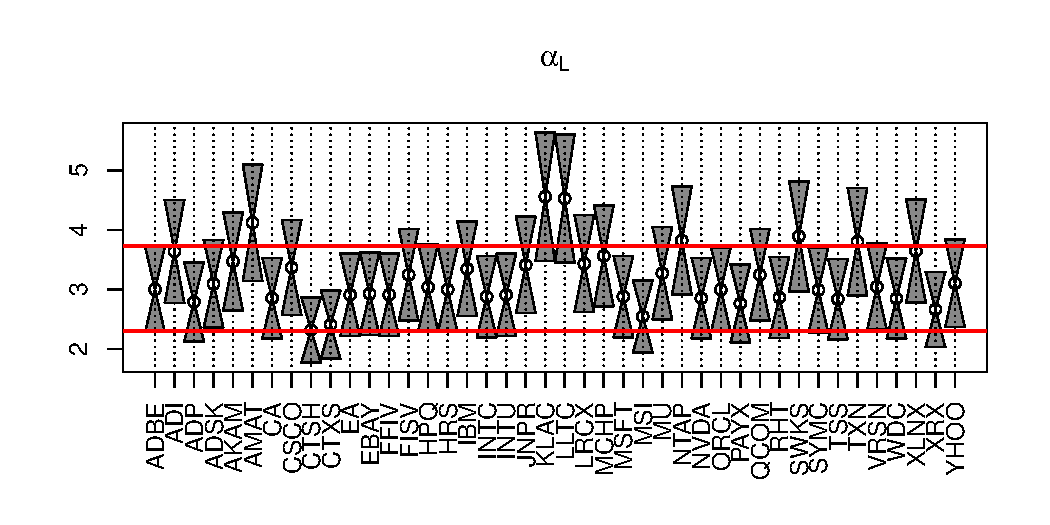
\includegraphics[width=\textwidth, trim={0, 0.8cm, 0, 2cm}, clip]
    {Information_Technology_lower.pdf}
  \end{minipage}
  \caption{\small Hill estimates $\hat \alpha_{50}$ of the lower
    tail-indices $\alpha$ of daily return series in sectors of the S\&P 500
    index. The data span from 1 January 2010 to 31 December 2014 and
    comprise $n=1304$ observations.
    The graphs from top to bottom correspond to the ``Energy'',
    ``Consumer Staples'' and ``Information Technology'' sectors.
    Each circle corresponds to a Hill estimate $\hat\alpha_{50}$; the gray
    triangles above and below it mark the 97.5\% and 2.5\% quantiles
    of its approximate normal distribution; see \eqref{eq:2} and the
    discussion following it for an interpretation.
    The lower and upper red lines mark the medians of the 2.5\% 
    and 97.5\% quantiles, respectively, evaluated from all stocks in
    the sector.
    The data are taken from {\it Yahoo Finance}; the labels on
    the horizontal axes are Yahoo symbols of the stocks. 
  }\label{fig:thjyuj}
\end{figure}

Random variables with regularly varying tails have some very nice
features: if $X_1$ and $X_2$ are both regularly varying with indices
$\alpha_1$ and $\alpha_2$, respectively, then $a_1 X_1 + a_2 X_2$ is
regularly varying with index $\min\{\alpha_1,
\alpha_2\}$ (cf. Mikosch and Jessen
\cite{JessenMikosch2006}). Moreover, if $X_1, X_2$ are iid,
$\P(a_1 X_1 + a_2 X_2 > u) \sim \P(a_1 X_1 > u) + \P(a_2 X_2 > u)$.

Now consider $p$ return series
$X_{i,t}$, $i=1,2,\dots, p; t=1,\dots,n$.
Suppose each of these series is a linear combination of $K$ factors
$Y_{j,t}$, $j=1,2,\dots,K$, the $j$-th of which is regularly varying
with index $\alpha_j$. Then by the summation property, each and every
$X_i$ is regularly varying with index $\min_{1 \leq j \leq K} \alpha_j$.
In practice a factor $Y_{i,t}$ is estimated as
$\hat Y_{j,t} = \sum_{i=1}^p a_{j, i} X_{i,t}$, where
$(a_{j, 1}, a_{j, 2}, \dots, a_{j, p})^\top$ is the $j$-th eigenvector
of the sample covariance matrix of
$\{X_{i,t}\}, i=1,\dots,p; t=1,\dots,n$, i.e. the eigenvector
associated with the $j$-th largest eigenvalue. 
For this reason, it is important to understand the eigensystem of the
sample covariance matrix of $\{X_{i,t}\}$. This topic is addressed in
chapters \ref{ch:bernoulli} and \ref{ch:extremes} of this thesis.

When a product of positive random variables, say $X_1 X_2$, involves
one with regularly varying tails, a useful result is that of
Breiman \cite{breiman:1965}: assume $X_1$ is regularly varying with
index $\alpha$ and there exists $\epsilon > 0$ such that
$\E X_2^{\alpha + \epsilon} < \infty$.
Then $\P(X_1 X_2 > x) \sim \E X_2^{\alpha} \P(X_1 > x)$.
More generally, if $X_1, X_2$ are regularly varying with the same tail
index $\alpha$ or if $\P(X_2 > x) = o(\P(X_1 > x))$, then $X_1 X_2$ is
regularly varying with index $\alpha$.

For an extensive summary of the regular variation properties of
functions of regularly varying random variables, see Mikosch and
Jessen \cite{JessenMikosch2006}.

% When considered as the multiplicative inverse of the parameter of the
% {\em Generalized Extreme Value} distribution, there are other methods
% in the literature for estimating the tail index, e.g. Pickand's 
% estimator \cite{pickands1975statistical} $\hat \alpha_P$ and the
% Deckers-Einmahl-de Haan estimator $\hat \alpha_{\text{DEH}}$
% \begin{eqnarray*}
% {1 \over \hat \alpha_P}
% &=&
% {1 \over \log 2}
% \log {
%   X_{(k)} - X_{(2k)}
%   \over
% X_{(2k)} - X_{(4k)}  
% } \\
% {1 \over \hat \alpha_{\text{DEH}}}
% &=&
% 1 + {1 \over \alpha_H} + {1 \over 2} \left(
%   {H \over \alpha_H^2} - 1
% \right)^{-1}
% \end{eqnarray*}
% where it is similarly assumed $k \to \infty$ and $k/n \to 0$ as $n \to
% \infty$. The Deckers-Einmahl-de Haan estimator makes use of Hill's
% estimator $\hat \alpha_H$ and computes
% \[
% H = \left[
%   {1 \over k} \sum_{i=1}^k \log \left(
%     { X_{(i)} \over X_{(k+1)} }
%   \right)^2
% \right]^{-1}
% \]
% Apparently $1/H$ can be interpreted as the 2nd empirical moment of
% $\log(X_{(i)}/X_{(k+1)})$ for $i \leq k$.
% A major drawback of Pickand's and Deckers-Einmahl-de Haan's estimators
% is that, when applied to estimating the tail index, they discard the
% information that the tail index is always positive, hence resulting in
% a larger confidence band compared with that obtained for Hill's
% estimator. Therefore we stick to Hill's estimator in the empirical
% work included in this thesis.

\section{Stochastic Recurrence Equation}
One of the most important dynamical mechanisms that lead to regularly
varying r.v. is stochastic recursion of the following form:
\begin{equation}
  \label{eq:rhjyu}
  X_t = A_t X_{t-1} + B_t, \quad t \in \mathbb Z
\end{equation}
where $X_t$ is a $d$-dimensional random vector, $A_t$ is a $d\times d$
random matrix and $B_t$ is a $d$-dimensional vector, random or
deterministic. The sequence $\{(A_t, B_t)\}_{t \in \mathbb Z}$ are
iid. The stationary solution to \eqref{eq:rhjyu} satisfies the fixed-point
equation $X \overset{d}{=} A X + B$, where $X$ and $(A, B)$ are
generic elements of the $\{X_t\}_{t \in \mathbb Z}$ and
$(A_t, B_t)_{t \in \mathbb Z}$ sequences.

Kesten \cite{kesten:1973} showed that, when $A_t$ are almost
surely non-negative, has no row or column of only zeros, and
$B_t$ is almost surely non-negative and is not equal to the null
vector with probability 1, then the solution $X$ to the equation
$X \overset{d}{=} A X + B$ is regularly varying with a positive index
$\alpha$, assuming the following conditions (M) and (A):
\begin{itemize}
\item Condition (M)
  \begin{enumerate}
  \item The top Lyapunov exponent
    \[
    \gamma = \inf_{n \geq 1} {1 \over n}\E \log \|A_n \cdots A_1\|
    \]
    is negative.
  \item There exists $\alpha > 0$ such that
    \[
    1 = \lambda(\alpha) = \lim_{n \to \infty} {1 \over n} \log \E \|A_n \cdots A_1\|^\alpha
    \]
  \item $\E (\|A_1\|^\alpha \log^+\|A_1\|) < \infty$
  \item $\E |B_1|^\alpha < \infty$
  \end{enumerate}
\item Condition (A) : The group generated by
  \[
  \{\log\rho(s): s = A_n \cdots A_1 \text{ for some } n \geq 1\}
  \]
  is dense in $\reals$, where $\rho(s)$ denotes the spectral
  radius of matrix $s$.
\end{itemize}
Upon these conditions, Kesten's theorem gives
\begin{equation*}
  u^\alpha \P(u^{-1} V \in \cdot) \overset{v}{\to} \nu_\alpha(\cdot)
\end{equation*}
where $\nu_\alpha$ is a non-null Radon measure on
$\reals^d_+ \setminus \{0\}$ with the property
$\nu_\alpha(a A) = a^{-\alpha} \nu_\alpha(A)$.

\section{GARCH models}
Introduced by Bollerslev \cite{bollerslev:1986} in 1986,
{\em Generalized Autoregressive Conditional Heteroscedasticity}
(GARCH) models have been hugely popular for modelling volatility of
financial time series and have inspired numerous variants.
A GARCH($p, q$) model is a stationary process
$\{X_t\}_{t \in \mathbb Z}$satisfying
\begin{eqnarray*}
  X_t &=& \sigma_t Z_t \\
  \sigma_t^2 &=& \omega + \sum_{i=1}^p \alpha_i X_{t-i}^2 +
  \sum_{j=1}^q \beta_j \sigma_{t-j}^2
\end{eqnarray*}
where $\{X_t\}$ is a return series, e.g. stock returns, foreign exchange
rates, interest rates, etc; $\{Z_t\}$ is a iid, mean 0, unit-variance
sequence; and $\sigma_t^2$ is the variance of the
distribution of $X_t$ conditional on $\{(X_i,
\sigma_i^2)\}_{i=0}^{t-1}$; $\omega, \{\alpha_i\}_{i=1}^p,
\{\beta_i\}_{i=1}^q$ are non-negative parameters of the
model. The GARCH($p,q$) recurrence equation is of the form of
\eqref{eq:rhjyu}. With appropriate conditions, $\sigma_t^2$ is
shown to be a positive Harris recurrent Markov chain (cf. Bollerslev
\cite{bollerslev:1986} and Buraczewski et al.
\cite{buraczewski:damek:mikosch:2016}), whose stationary distribution
has regularly varying tails. The tail index $\alpha$, is given by
\begin{equation}
  \label{eq:grgbg}
  \lim_{n \to \infty} {1 \over n}\log\E\|A_n \cdots A_1\|^\alpha = 0,
\end{equation}
where $\{A_i\}_{i \in \mathbb Z}$ are iid matrices whose entries are
functions of $\{\alpha_i\}_{i=1}^p$, $\{\beta_i\}_{i=1}^q$ and
$\{Z_t^2\}$:
\[
A_i =
\begin{pmatrix}
  \alpha_1 Z_{t-1}^2 + \beta_1 & \beta_2 & \cdots &
  \beta_{q-1} & \beta_q & \alpha_2 & \alpha_3 &
  \cdots & \alpha_{p-1} & \alpha_p\\
  1 & 0 & \cdots & 
  0 & 0 & 0 & 0 & \cdots & 0 & 0 \\
  \vdots & \vdots & \ddots & 
  \vdots & \vdots & \vdots & \vdots &
  \ddots & \vdots & \vdots \\
  0 & 0 & \cdots &
  0 & 0 & 0 & 0 & \cdots & 0 & 0 \\
  0 & 0 & \cdots &
  1 & 0 & 0 & 0 & \cdots & 0 & 0 \\
  Z_{t-1}^2 & 0 & \cdots &
  0 & 0 & 0 & 0 & \cdots & 0 & 0 \\
  0 & 0 & \cdots &
  0 & 0 & 1 & 0 & \cdots & 0 & 0 \\
  \vdots & \vdots & \ddots &
  \vdots & \vdots & \vdots & \vdots &
  \ddots & \vdots & \vdots \\
  0 & 0 & \cdots &
  0 & 0 & 0 & 0 & \cdots & 0 & 0 \\    
  0 & 0 & \cdots &
  0 & 0 & 0 & 0 & \cdots & 1 & 0 \\    
\end{pmatrix}
\]
While GARCH models have been very successful for modelling financial
time series, it does have its drawbacks. For example, the tail
index is very sensitive to the model parameters $\{\alpha_i\}_{i=1}^p$ and
$\{\beta_i\}_{i=1}^q$. In applications, these parameters need to be
estimated from a sample and are all ways uncertain to an extent, there
can be a significant discrepancy between the tail index implied by
\eqref{eq:grgbg} and the Hill estimate \eqref{eq:fhhty}.

There exist various extensions of the univariate GARCH
model to the multivariate case. The most notable one is perhaps the
{\em constant conditional correlation} (CCC) model of Bollerslev
\cite{bollerslev:1990} and Jeantheau \cite{jeantheau:1998}. In the
bivariate case, CCC is the model 
\beao\bfX_t=
\left(\barr{l}X_{1,t}\\
X_{2,t}\earr\right)= \left(\barr{ll}\sigma_{1,t}& 0\\
0&\sigma_{2,t}\earr\right)\,\left(\barr{l}Z_{1,t}\\Z_{2,t}\earr\right)=\Sigma_t\,\bfZ_t\,,\qquad
t\in\bbz\,.
\eeao
Thus both return components $X_{i,t}$ have the form of a univariate
stochastic volatility model $X_{i,t}=\sigma_{i,t}Z_{i,t}$ 
with non-negative volatility $\sigma_{i,t}$ and an iid bivariate noise
\seq\ $(\bfZ_t)$ with zero mean and unit variance components.
We also have the specification
\begin{small}
\beam\label{eq:8:mikosch}
\bfY_t=\left(\barr{l}\sigma^2_{1,t}  \\  
\sigma^2_{2,t}\earr
\right)
&=& \left(
\barr{l}\alpha_{01}  \\\alpha_{02}   \earr\right)
+\left(\barr{cc}\alpha_{11} & \alpha_{12}  \\
      \alpha_{21} & \alpha_{22}\earr \right)\, 
\left(\barr{l}X_{1,t-1}^2  \\X_{2,t-1}^2   \earr\right)
 + \left(\barr{cc}\beta_{11} & \beta_{12}  \\\beta_{21} & \beta_{22} \earr
 \right)\,\left(\barr{c}\sigma^2_{1,t-1}  \\\sigma^2_{2,t-1}\earr
  \right)\nonumber\\
&=& \left(
\barr{l}\alpha_{01}  \\\alpha_{02}
\earr\right)+\left(\barr{cc}\alpha_{11}Z_{1,t-1}^2+\beta_{11}&\alpha_{12}Z_{2,t-1}^2+
\beta_{12}\\
\alpha_{21}Z_{1,t-1}^2+\beta_{21}& \alpha_{22}Z_{2,t-1}^2+\beta_{22}
\earr\right)\,\left(\barr{l}\sigma_{1,t-1}^2\\\sigma_{2,t-1}^2\earr
\right)\,,
\eeam
for positive $\alpha_{0i}$ and suitable non-negative 
$\alpha_{ij},\beta_{ij}$, $i,j=1,2$.
Writing
\beao
\bfB_t= \left(
\barr{l}\alpha_{01}  \\\alpha_{02}   \earr\right)\quad\mbox{and}\quad
\bfA_t=\left(\barr{cc}\alpha_{11}Z_{1,t-1}^2+\beta_{11}&\alpha_{12}Z_{2,t-1}^2+
\beta_{12}\\
\alpha_{21}Z_{1,t-1}^2+\beta_{21}& \alpha_{22}Z_{2,t-1}^2+\beta_{22}
\earr\right)\,,
\eeao
\end{small}
we see that we are again in the framework of a stochastic recurrence equation\ 
but this time for vector-valued $\bfB_t$ and matrix-valued $\bfA_t$:
\beam\label{eq:jan6b:mikosch}
\bfY_t=\bfA_t\,\bfY_{t-1}+\bfB_t\,,\qquad t\in\bbz\,.
\eeam
Kesten \cite{kesten:1973} also provided the corresponding theory  
for stationarity and tails in this case. \sta\ \cite{starica:1999}
dealt with the corresponding problems for CCC-GARCH processes,
making use of the theory in Kesten \cite{kesten:1973},
Bougerol and Picard \cite{bougerol:picard:1992}
and its
specification to the tails of GARCH models 
in Basrak et al.~\cite{basrak:davis:mikosch:2002}. \sta\ \cite{starica:1999} assumed the 
Kesten conditions for the matrices $\bfA_t$. These conditions ensure
that the product matrices $\bfA_1\cdots\bfA_n$ have positive entries
for sufficiently large $n$. Then Kesten's theory implies that all
components of the vector $\bfX_t$ have power-law tails with the same
index $\alpha$ and also that the \fidi s of the process $(\bfX_t)$ are
\regvary\ with index $\alpha$.
\par
Various GARCH modifications are derived by considering linear
combinations of CCC-GARCH models. The property of multivariate
\regvar\ of multivariate GARCH ensures that, after linear
transformations,  the new process in all components has again
power-law tails with the same index as the original GARCH process; see
Basrak et al.~\cite{basrak:davis:mikosch:2002}.
Models which are constructed in this way are
the Orthogonal GARCH model of
Alexander and Chibumba \cite{alexander:chibumba:1996}, its
generalization GO-GARCH by van der Weide \cite{Weide2002},  the Full
Factor GARCH model of Vrontos et al. \cite{vrontos2003full} and the
Generalized Orthogonal Factor GARCH model of Lanne and Saikkonen
\cite{lanne2007modelling}. These models are characterized by their
treatment of each series as a linear combination of factors, and each
of the factors is modeled as a GARCH process; see Silvennoinen and
Ter\"asvirt\"a \cite{silventeras:2009}.
\par
Not all choices of $\alpha$- and $\beta$-parameters in the model
\eqref{eq:8:mikosch} allow for an application of the Kesten theory. For
example, assume that only the diagonal elements $\alpha_{ii}$ and
$\beta_{ii}$ are positive. Then $\bfA_t$ is diagonal and, hence, the
condition that $\bfA_1\cdots\bfA_n$ have positive entries for
sufficiently large $n$  cannot be satisfied. In the latter situation,
both $(X_{1,t})$ and $(X_{2,t})$ are univariate GARCH
processes. Assuming the  conditions of the univariate Kesten-Goldie
theorem for each component process, $(X_{1,t})$ and $(X_{2,t})$ have
power-law tails  with indices $\alpha_1$ and $\alpha_2$, respectively,
given by the solutions to the equations  $\E [(\alpha_{ii}
Z_{i,t}^2+\beta_{ii})^{\alpha_i/2}]=1$, $i=1,2$. In this model, one
can introduce dependence between the two component series $(X_{1,t})$
and $(X_{2,t})$ by assuming dependence between the noise variables
$Z_{1,t}$ and $Z_{2,t}$. Another situation when the Kesten theory fails 
appears when $\bfA_t$ is an upper or lower triangle matrix: then the
products  $\bfA_1\cdots\bfA_n$ are always of the same triangular
type. 
Similar remarks apply when one considers a CCC model in general
dimension. Of course, one may argue that the latter models 
are not natural: they are degenerate since they do not allow 
for a linear relationship between all squared volatilities on a given
day.

\section{Stochastic Volatility models}


\section{Contribution of this thesis}\label{sec:contr}

In this section we summarize our results from the research papers.

\subsection{Tail parameters of equity return series}
We have established that, in the case of an equity return series with
two-sided, functionally independent Pareto tails, investor
preference functionals are monotone increasing/decreasing with the
tail index/scale parameters. Thus in a market dominated by such
equities, the investors would pursue the largest tail index in the
market, leading to a shared common tail index for all equities.

The empirical results presented in section \ref{sec:1} suggest this
may well be the case for the ``Consumer Staples'' sector of S\&P 500,
given the Hill estimates of tail indices shown in figure \ref{fig:1}
and the largely positive results of tests for equal tail indices shown
in figure \ref{fig:PairTest}.

On the other hand, we have also seen that, when the left and the right
tails have the same indices, investor preference over the equity has
more sophisticated variations in the parameters' space including the
tail parameters of the equity, the interest rate, the investor's risk
apetite as captured by his utility function, and his threshold of
disappointment.

We also acknowledge that our model of the market and the investor is a
simple one, not accoounting for the dependence between equities, nor
the categorization of investors and their interactions. These are
potential topics of future work.

